\documentclass{standalone}
\usepackage{tikz}
\usetikzlibrary{patterns, positioning}
\usepackage[sfdefault]{ClearSans} %% option 'sfdefault' activates Clear Sans as the default text font
\usepackage[T1]{fontenc}

\begin{document}
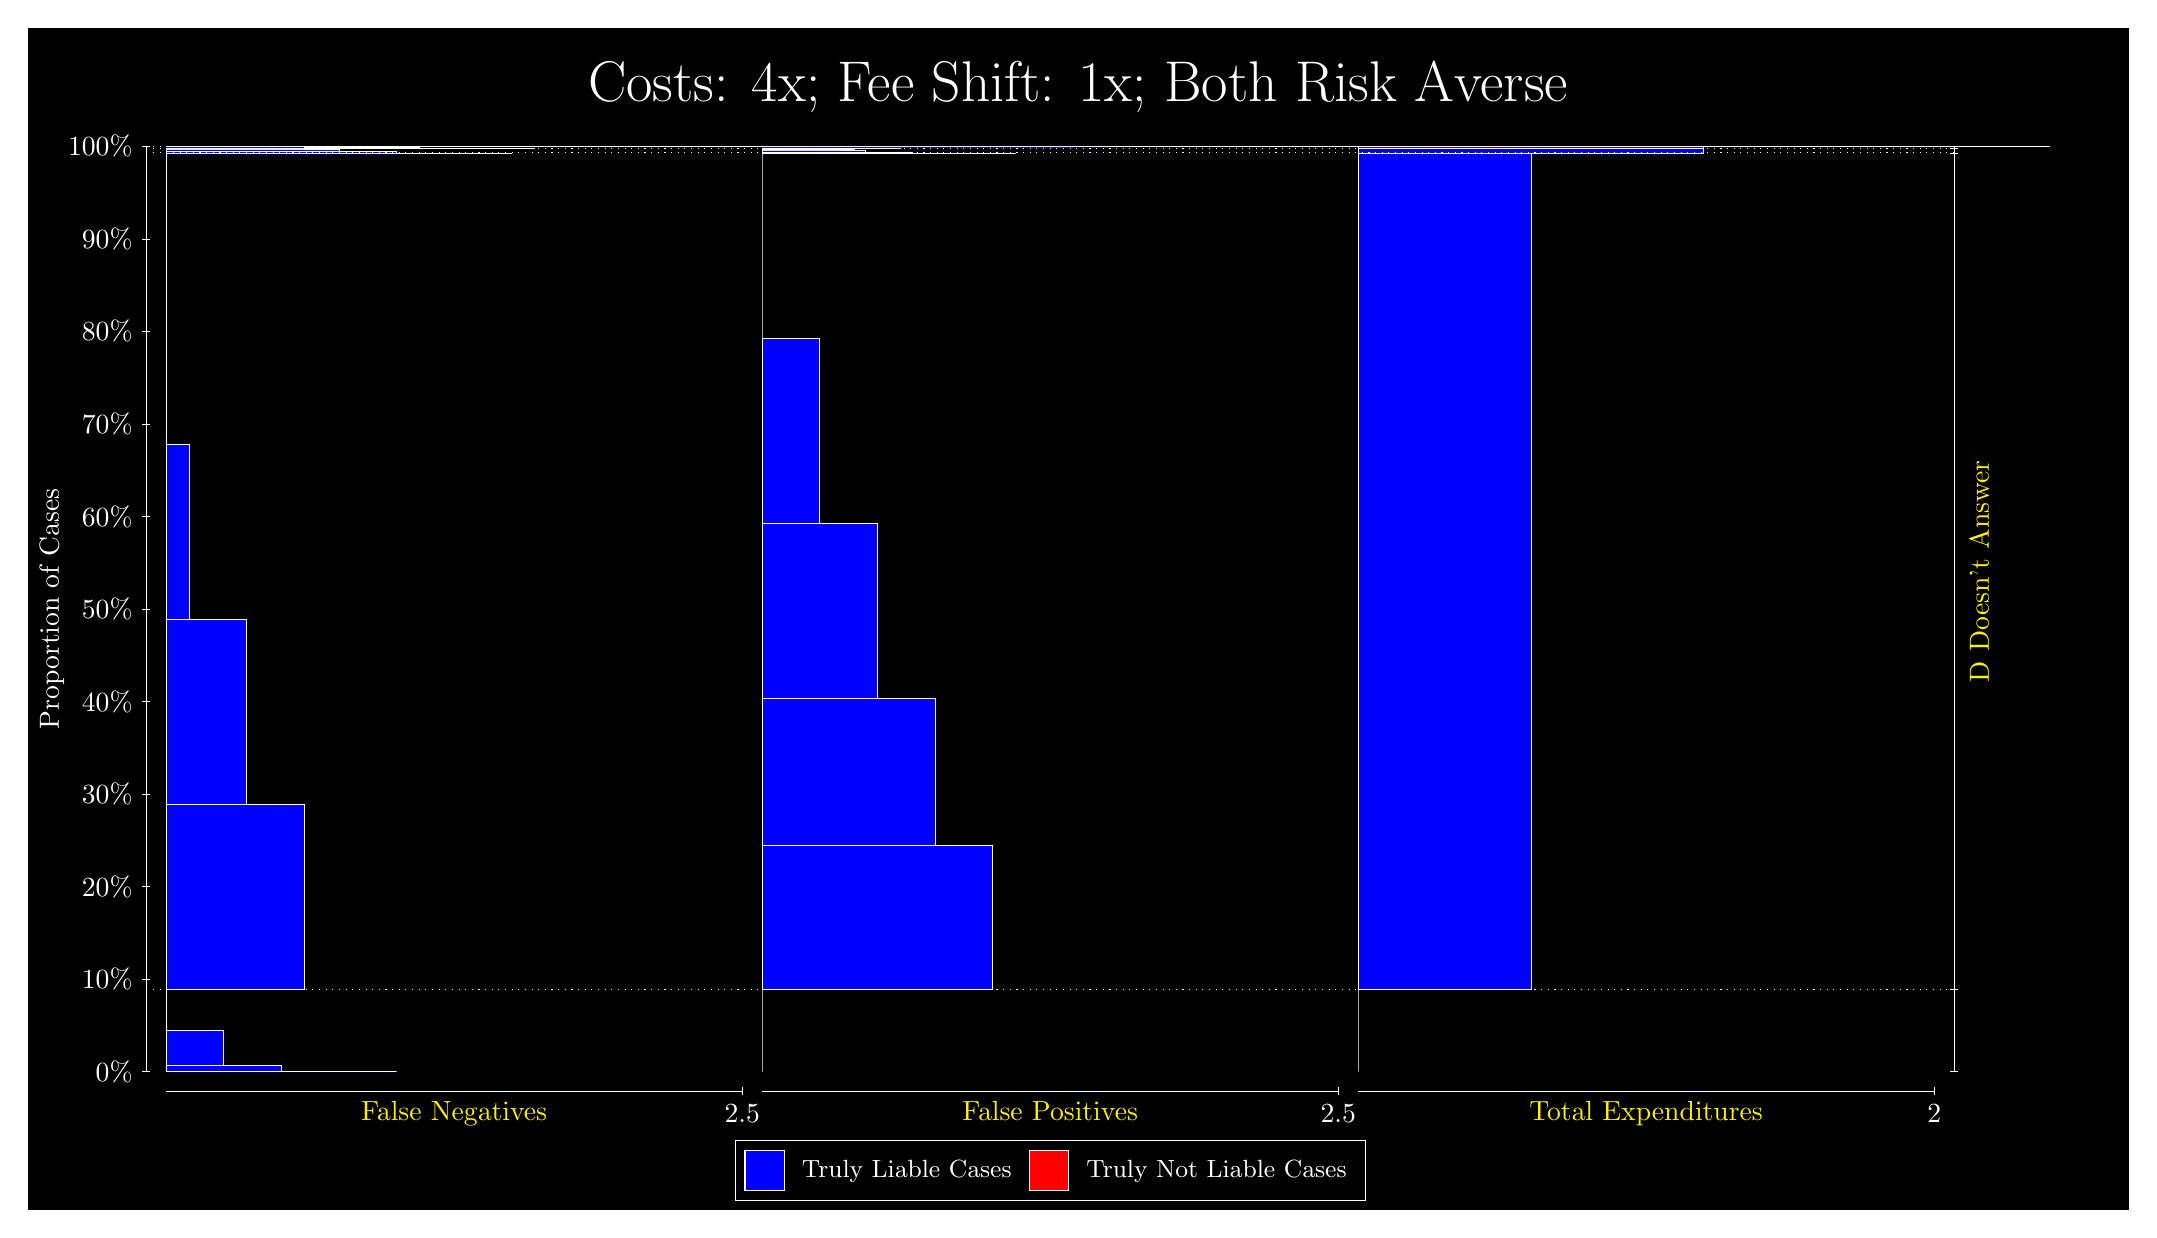
\begin{tikzpicture}
\draw[fill=black] (0,0) rectangle (26.667,15);
\draw[text=white] (0,13.5) rectangle (26.667,15) node[midway] {\huge Costs: 4x; Fee Shift: 1x; Both Risk Averse};
\draw[white, very thin] (1.5,1.75) -- (1.5,13.5);
\node[rotate=90, text=white, anchor=center] at (0.3, 7.625) {Proportion of Cases};
\draw[white, very thin] (1.45,1.75) -- (1.55,1.75);
\node[text=white, anchor=east] at (1.45, 1.75) {0\%};
\draw[white, very thin] (1.45,2.925) -- (1.55,2.925);
\node[text=white, anchor=east] at (1.45, 2.925) {10\%};
\draw[white, very thin] (1.45,4.1) -- (1.55,4.1);
\node[text=white, anchor=east] at (1.45, 4.1) {20\%};
\draw[white, very thin] (1.45,5.275) -- (1.55,5.275);
\node[text=white, anchor=east] at (1.45, 5.275) {30\%};
\draw[white, very thin] (1.45,6.45) -- (1.55,6.45);
\node[text=white, anchor=east] at (1.45, 6.45) {40\%};
\draw[white, very thin] (1.45,7.625) -- (1.55,7.625);
\node[text=white, anchor=east] at (1.45, 7.625) {50\%};
\draw[white, very thin] (1.45,8.8) -- (1.55,8.8);
\node[text=white, anchor=east] at (1.45, 8.8) {60\%};
\draw[white, very thin] (1.45,9.975) -- (1.55,9.975);
\node[text=white, anchor=east] at (1.45, 9.975) {70\%};
\draw[white, very thin] (1.45,11.15) -- (1.55,11.15);
\node[text=white, anchor=east] at (1.45, 11.15) {80\%};
\draw[white, very thin] (1.45,12.325) -- (1.55,12.325);
\node[text=white, anchor=east] at (1.45, 12.325) {90\%};
\draw[white, very thin] (1.45,13.5) -- (1.55,13.5);
\node[text=white, anchor=east] at (1.45, 13.5) {100\%};

\draw[white, very thin] (24.457,1.75) -- (24.457,13.5);
\draw[white, very thin] (24.407,1.75) -- (24.507,1.75);
\node[anchor=west] at (24.407, 1.75) {};
\draw[white, very thin] (24.407,2.7942) -- (24.507,2.7942);
\node[anchor=west] at (24.407, 2.7942) {};
\draw[white, very thin] (24.407,13.416) -- (24.507,13.416);
\node[anchor=west] at (24.407, 13.416) {};
\draw[white, very thin] (24.407,13.478) -- (24.507,13.478);
\node[anchor=west] at (24.407, 13.478) {};
\draw[white, very thin] (24.407,13.496) -- (24.507,13.496);
\node[anchor=west] at (24.407, 13.496) {};
\draw[white, very thin] (24.407,13.5) -- (24.507,13.5);
\node[anchor=west] at (24.407, 13.5) {};
\draw[white, very thin] (24.407,13.5) -- (24.507,13.5);
\node[anchor=west] at (24.407, 13.5) {};

\draw[white, very thin, fill=blue] (1.75,1.75) rectangle (4.6775,1.75);
\draw[white, very thin, fill=blue] (1.75,1.75) rectangle (3.9457,1.7507);
\draw[white, very thin, fill=blue] (1.75,1.7507) rectangle (3.2138,1.8336);
\draw[white, very thin, fill=blue] (1.75,1.8336) rectangle (2.4819,2.2728);
\draw[white, very thin, fill=red] (1.75,2.2728) rectangle (1.75,2.2728);
\draw[white, very thin, fill=blue] (1.75,2.2728) rectangle (1.75,2.7942);
\draw[white, very thin, fill=blue] (1.75,2.7942) rectangle (3.5065,5.1441);
\draw[white, very thin, fill=blue] (1.75,5.1441) rectangle (2.7746,7.4931);
\draw[white, very thin, fill=blue] (1.75,7.4931) rectangle (2.0428,9.7215);
\draw[white, very thin, fill=red] (1.75,9.7215) rectangle (1.75,9.7215);
\draw[white, very thin, fill=blue] (1.75,9.7215) rectangle (1.75,13.416);
\draw[white, very thin, fill=blue] (1.75,13.416) rectangle (6.1413,13.416);
\draw[white, very thin, fill=blue] (1.75,13.416) rectangle (5.8486,13.416);
\draw[white, very thin, fill=blue] (1.75,13.416) rectangle (5.5558,13.416);
\draw[white, very thin, fill=blue] (1.75,13.416) rectangle (5.4094,13.416);
\draw[white, very thin, fill=blue] (1.75,13.416) rectangle (5.2631,13.416);
\draw[white, very thin, fill=blue] (1.75,13.416) rectangle (5.1167,13.416);
\draw[white, very thin, fill=blue] (1.75,13.416) rectangle (4.9703,13.416);
\draw[white, very thin, fill=blue] (1.75,13.416) rectangle (4.8239,13.416);
\draw[white, very thin, fill=blue] (1.75,13.416) rectangle (4.6775,13.434);
\draw[white, very thin, fill=blue] (1.75,13.434) rectangle (4.5312,13.434);
\draw[white, very thin, fill=blue] (1.75,13.434) rectangle (4.3848,13.437);
\draw[white, very thin, fill=blue] (1.75,13.437) rectangle (4.2384,13.437);
\draw[white, very thin, fill=blue] (1.75,13.437) rectangle (4.092,13.443);
\draw[white, very thin, fill=blue] (1.75,13.443) rectangle (3.9457,13.466);
\draw[white, very thin, fill=blue] (1.75,13.466) rectangle (3.7993,13.467);
\draw[white, very thin, fill=blue] (1.75,13.467) rectangle (3.6529,13.47);
\draw[white, very thin, fill=blue] (1.75,13.47) rectangle (3.5065,13.47);
\draw[white, very thin, fill=blue] (1.75,13.47) rectangle (3.3602,13.477);
\draw[white, very thin, fill=blue] (1.75,13.477) rectangle (3.2138,13.478);
\draw[white, very thin, fill=blue] (1.75,13.478) rectangle (3.0674,13.478);
\draw[white, very thin, fill=blue] (1.75,13.478) rectangle (2.921,13.478);
\draw[white, very thin, fill=blue] (1.75,13.478) rectangle (2.7746,13.478);
\draw[white, very thin, fill=blue] (1.75,13.478) rectangle (2.6283,13.478);
\draw[white, very thin, fill=blue] (1.75,13.478) rectangle (2.3355,13.478);
\draw[white, very thin, fill=blue] (1.75,13.478) rectangle (2.0428,13.478);
\draw[white, very thin, fill=red] (1.75,13.478) rectangle (1.75,13.478);
\draw[white, very thin, fill=blue] (1.75,13.478) rectangle (6.4341,13.478);
\draw[white, very thin, fill=blue] (1.75,13.478) rectangle (5.7022,13.478);
\draw[white, very thin, fill=blue] (1.75,13.478) rectangle (4.9703,13.486);
\draw[white, very thin, fill=blue] (1.75,13.486) rectangle (4.2384,13.495);
\draw[white, very thin, fill=blue] (1.75,13.495) rectangle (3.5065,13.496);
\draw[white, very thin, fill=red] (1.75,13.496) rectangle (1.75,13.496);
\draw[white, very thin, fill=blue] (1.75,13.496) rectangle (3.5065,13.496);
\draw[white, very thin, fill=blue] (1.75,13.496) rectangle (2.7746,13.496);
\draw[white, very thin, fill=blue] (1.75,13.496) rectangle (2.0428,13.499);
\draw[white, very thin, fill=red] (1.75,13.499) rectangle (1.75,13.499);
\draw[white, very thin, fill=blue] (1.75,13.499) rectangle (1.75,13.5);
\draw[white, very thin, fill=blue] (1.75,13.5) rectangle (11.704,13.5);
\draw[white, very thin, fill=blue] (1.75,13.5) rectangle (10.972,13.5);
\draw[white, very thin, fill=blue] (1.75,13.5) rectangle (10.24,13.5);
\draw[white, very thin, fill=blue] (1.75,13.5) rectangle (9.508,13.5);
\draw[white, very thin, fill=blue] (1.75,13.5) rectangle (8.7761,13.5);
\draw[white, very thin, fill=blue] (1.75,13.5) rectangle (8.0442,13.5);
\draw[white, very thin, fill=blue] (1.75,13.5) rectangle (3.9457,13.5);
\draw[white, very thin, fill=blue] (1.75,13.5) rectangle (3.2138,13.5);
\draw[white, very thin, fill=blue] (1.75,13.5) rectangle (2.4819,13.5);
\draw[white, very thin, fill=red] (1.75,13.5) rectangle (1.75,13.5);
\draw[white, very thin, fill=blue] (1.75,13.5) rectangle (1.75,13.5);
\draw[white, very thin, fill=red] (9.3189,1.75) rectangle (9.3189,1.75);
\draw[white, very thin, fill=blue] (9.3189,1.75) rectangle (9.3189,2.7942);
\draw[white, very thin, fill=red] (9.3189,2.7942) rectangle (12.246,2.7942);
\draw[white, very thin, fill=blue] (9.3189,2.7942) rectangle (12.246,4.6221);
\draw[white, very thin, fill=blue] (9.3189,4.6221) rectangle (11.515,6.4884);
\draw[white, very thin, fill=blue] (9.3189,6.4884) rectangle (10.783,8.7169);
\draw[white, very thin, fill=blue] (9.3189,8.7169) rectangle (10.051,11.066);
\draw[white, very thin, fill=blue] (9.3189,11.066) rectangle (9.3189,13.416);
\draw[white, very thin, fill=red] (9.3189,13.416) rectangle (12.539,13.416);
\draw[white, very thin, fill=blue] (9.3189,13.416) rectangle (12.539,13.416);
\draw[white, very thin, fill=red] (9.3189,13.416) rectangle (12.246,13.416);
\draw[white, very thin, fill=blue] (9.3189,13.416) rectangle (12.246,13.416);
\draw[white, very thin, fill=red] (9.3189,13.416) rectangle (11.954,13.416);
\draw[white, very thin, fill=blue] (9.3189,13.416) rectangle (11.954,13.416);
\draw[white, very thin, fill=blue] (9.3189,13.416) rectangle (11.807,13.416);
\draw[white, very thin, fill=red] (9.3189,13.416) rectangle (11.661,13.416);
\draw[white, very thin, fill=blue] (9.3189,13.416) rectangle (11.661,13.416);
\draw[white, very thin, fill=blue] (9.3189,13.416) rectangle (11.515,13.416);
\draw[white, very thin, fill=red] (9.3189,13.416) rectangle (11.368,13.416);
\draw[white, very thin, fill=blue] (9.3189,13.416) rectangle (11.368,13.417);
\draw[white, very thin, fill=blue] (9.3189,13.417) rectangle (11.222,13.423);
\draw[white, very thin, fill=blue] (9.3189,13.423) rectangle (11.075,13.424);
\draw[white, very thin, fill=blue] (9.3189,13.424) rectangle (10.929,13.427);
\draw[white, very thin, fill=blue] (9.3189,13.427) rectangle (10.783,13.428);
\draw[white, very thin, fill=blue] (9.3189,13.428) rectangle (10.636,13.451);
\draw[white, very thin, fill=blue] (9.3189,13.451) rectangle (10.49,13.457);
\draw[white, very thin, fill=blue] (9.3189,13.457) rectangle (10.344,13.457);
\draw[white, very thin, fill=blue] (9.3189,13.457) rectangle (10.197,13.46);
\draw[white, very thin, fill=blue] (9.3189,13.46) rectangle (10.051,13.46);
\draw[white, very thin, fill=blue] (9.3189,13.46) rectangle (9.9044,13.478);
\draw[white, very thin, fill=blue] (9.3189,13.478) rectangle (9.758,13.478);
\draw[white, very thin, fill=blue] (9.3189,13.478) rectangle (9.6116,13.478);
\draw[white, very thin, fill=blue] (9.3189,13.478) rectangle (9.4652,13.478);
\draw[white, very thin, fill=blue] (9.3189,13.478) rectangle (9.3189,13.478);
\draw[white, very thin, fill=red] (9.3189,13.478) rectangle (11.075,13.478);
\draw[white, very thin, fill=blue] (9.3189,13.478) rectangle (11.075,13.479);
\draw[white, very thin, fill=blue] (9.3189,13.479) rectangle (10.344,13.488);
\draw[white, very thin, fill=blue] (9.3189,13.488) rectangle (9.6116,13.495);
\draw[white, very thin, fill=blue] (9.3189,13.495) rectangle (9.3189,13.496);
\draw[white, very thin, fill=red] (9.3189,13.496) rectangle (14.003,13.496);
\draw[white, very thin, fill=blue] (9.3189,13.496) rectangle (14.003,13.496);
\draw[white, very thin, fill=blue] (9.3189,13.496) rectangle (13.271,13.497);
\draw[white, very thin, fill=blue] (9.3189,13.497) rectangle (12.539,13.5);
\draw[white, very thin, fill=blue] (9.3189,13.5) rectangle (11.807,13.5);
\draw[white, very thin, fill=blue] (9.3189,13.5) rectangle (11.075,13.5);
\draw[white, very thin, fill=red] (9.3189,13.5) rectangle (19.273,13.5);
\draw[white, very thin, fill=blue] (9.3189,13.5) rectangle (19.273,13.5);
\draw[white, very thin, fill=red] (9.3189,13.5) rectangle (18.541,13.5);
\draw[white, very thin, fill=blue] (9.3189,13.5) rectangle (18.541,13.5);
\draw[white, very thin, fill=red] (9.3189,13.5) rectangle (17.809,13.5);
\draw[white, very thin, fill=blue] (9.3189,13.5) rectangle (17.809,13.5);
\draw[white, very thin, fill=red] (9.3189,13.5) rectangle (17.077,13.5);
\draw[white, very thin, fill=blue] (9.3189,13.5) rectangle (17.077,13.5);
\draw[white, very thin, fill=blue] (9.3189,13.5) rectangle (16.345,13.5);
\draw[white, very thin, fill=blue] (9.3189,13.5) rectangle (15.613,13.5);
\draw[white, very thin, fill=blue] (9.3189,13.5) rectangle (14.881,13.5);
\draw[white, very thin, fill=blue] (9.3189,13.5) rectangle (14.149,13.5);
\draw[white, very thin, fill=red] (9.3189,13.5) rectangle (10.051,13.5);
\draw[white, very thin, fill=blue] (9.3189,13.5) rectangle (10.051,13.5);
\draw[white, very thin, fill=red] (9.3189,13.5) rectangle (9.3189,13.5);
\draw[white, very thin, fill=blue] (9.3189,13.5) rectangle (9.3189,13.5);
\draw[white, very thin, fill=red] (16.888,1.75) rectangle (16.888,1.75);
\draw[white, very thin, fill=blue] (16.888,1.75) rectangle (16.888,2.7942);
\draw[white, very thin, fill=red] (16.888,2.7942) rectangle (19.083,2.7942);
\draw[white, very thin, fill=blue] (16.888,2.7942) rectangle (19.083,13.416);
\draw[white, very thin, fill=red] (16.888,13.416) rectangle (21.279,13.416);
\draw[white, very thin, fill=blue] (16.888,13.416) rectangle (21.279,13.417);
\draw[white, very thin, fill=red] (16.888,13.417) rectangle (21.279,13.417);
\draw[white, very thin, fill=blue] (16.888,13.417) rectangle (21.279,13.478);
\draw[white, very thin, fill=red] (16.888,13.478) rectangle (21.279,13.478);
\draw[white, very thin, fill=blue] (16.888,13.478) rectangle (21.279,13.496);
\draw[white, very thin, fill=red] (16.888,13.496) rectangle (21.279,13.496);
\draw[white, very thin, fill=blue] (16.888,13.496) rectangle (21.279,13.5);
\draw[white, very thin, fill=red] (16.888,13.5) rectangle (25.67,13.5);
\draw[white, very thin, fill=blue] (16.888,13.5) rectangle (25.67,13.5);
\draw[white, dotted] (1.5,2.7942) -- (24.457,2.7942);
\draw[white, dotted] (1.5,13.416) -- (24.457,13.416);
\draw[white, dotted] (1.5,13.478) -- (24.457,13.478);
\draw[white, dotted] (1.5,13.496) -- (24.457,13.496);
\draw[white, dotted] (1.5,13.5) -- (24.457,13.5);
\draw[white, very thin] (1.75,1.5) -- (9.0689,1.5);
\node[text=yellow, anchor=north] at (5.4094, 1.5) {False Negatives};
\draw[white, very thin] (9.0689,1.45) -- (9.0689,1.55);
\node[text=white, anchor=north] at (9.0689, 1.45) {2.5};

\draw[white, very thin] (9.3189,1.5) -- (16.638,1.5);
\node[text=yellow, anchor=north] at (12.978, 1.5) {False Positives};
\draw[white, very thin] (16.638,1.45) -- (16.638,1.55);
\node[text=white, anchor=north] at (16.638, 1.45) {2.5};

\draw[white, very thin] (16.888,1.5) -- (24.207,1.5);
\node[text=yellow, anchor=north] at (20.547, 1.5) {Total Expenditures};
\draw[white, very thin] (24.207,1.45) -- (24.207,1.55);
\node[text=white, anchor=north] at (24.207, 1.45) {2};


\node[text=yellow, centered, rotate=90] at (24.777, 8.105) {D Doesn't Answer};





\draw (12.978300999999998,1.5) node[draw=none] (baseCoordinate) {};
\begin{scope}[align=center]
        \matrix[scale=0.5, draw=white, below=0.5cm of baseCoordinate, nodes={draw}, column sep=0.1cm]{
            \node[rectangle, draw, minimum width=0.5cm, minimum height=0.5cm, fill=blue] {}; &
            \node[draw=none, font=\small, text=white] (B) {Truly Liable Cases}; &
            \node[rectangle, draw, minimum width=0.5cm, minimum height=0.5cm, fill=red] {}; &
            \node[draw=none, font=\small, text=white] (B) {Truly Not Liable Cases}; \\
            };
\end{scope}

\end{tikzpicture}
\end{document}